% ------------------------------------------------------------------------ %
% !TEX encoding = UTF-8 Unicode
% !TEX TS-program = pdflatex
% !TEX root = ../Tesi.tex
% !TEX spellcheck = it-IT
% ------------------------------------------------------------------------ %
%
% ------------------------------------------------------------------------ %
% 	STATO DELL'ARTE
% ------------------------------------------------------------------------ %
%
\chapter{State of the Art}
%
\label{cap:statoarte}
%
% ------------------------------------------------------------------------ %
%
\section{Android OS} \label{androidos}
\par As already mentioned in \ref{motivation}, the Android operating system is an open source OS developed by Google based on Linux kernel, that can be installed on many different kind of devices.\\
In this section i want to give to the reader the basic knowledge of the Android framework to understand why and how the operating system works.
\subsection{Brief History}  
\par
The Android era officially began on October 22nd, 2008, when the \textit{T-Mobile G1} launched in the United States \cite{verge2011android}.\\
At that moment the company of mountain view, Google, felt the need to create a new operating system which was able to be installed on most modern mobile phones of the time. To meet this need the Google engineers created an OS that was based on the Linux kernel, lightweight enough and ease to be used with simple hand gestures by touching the screen of the phone.\\

\begin{figure}[h]
	\centering
	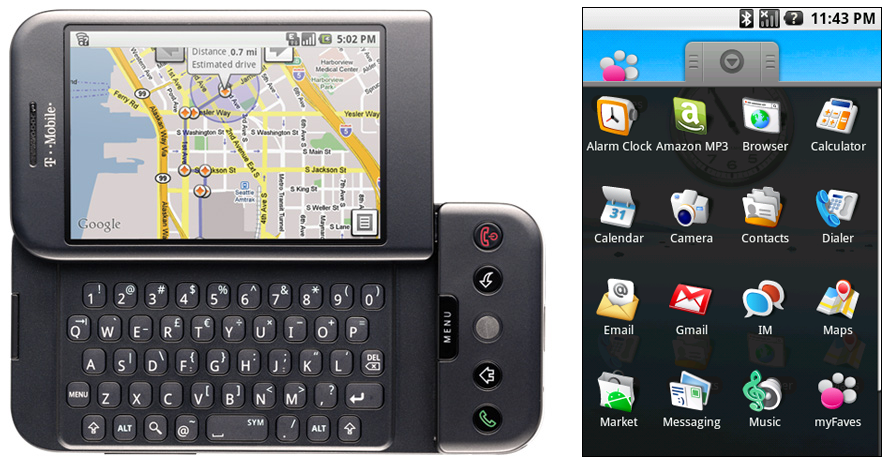
\includegraphics[width=0.8\textwidth]{T-MobileG1Android1menu}
	\caption{The T-Mobile G1 and the Android 1.0 menù}
	\label{2.1:The T-Mobile G1 and the Android 1.0 menù}
\end{figure}

The main characteristic of the OS were and are also now:
\begin{itemize}
	\item The pull-down notification window.
	\item Home screen widgets.
	\item The Android Market.
	\item Google services integration (eg. Gmail).
	\item Wireless connection technologies (eg Wi-Fi and Bluetooth)
\end{itemize}
The success of the first version of the brand new mobile operating system and the open source philosophy guaranteed the fast spread of the Android devices all over the world. In few years Google improved and released many version of the OS and with the help of the market growth Android has become a complete os. 
In the table below there is a brief description of the various distribution of the Android OS at the time of writing of this document.\\
\begin{table}[h]
	%
	\caption{Android versions}
	%
	\label{tab:vers}
	%
	\centering
	%
	\begin{tabular}{llll}
		%
		\toprule
		%
		\textbf{Name} & \textbf{Version}  & \textbf{Release Date} & \textbf{API Level}\\
		%
		\midrule
		%
		Alpha &	1.0 & September 23, 2008 & 1 \\
		Beta & 1.1 & February 9, 2009 & 2 \\
		Cupcake & 1.5 & April 27, 2009 & 3 \\
		Donut &	1.6 & September 15, 2009 & 4 \\
		Eclair & 2.0 – 2.1 & October 26, 2009 & 5–7 \\
		Froyo & 2.2 – 2.2.3 & May 20, 2010 & 8 \\
		Gingerbread & 2.3 – 2.3.7 & December 6, 2010 & 9–10 \\	
		Honeycomb & 3.0 – 3.2.6 & February 22, 2011 & 11–13 \\
		Ice Cream Sandwich & 4.0 – 4.0.4 & October 18, 2011 & 14–15 \\
		Jelly Bean & 4.1 – 4.3.1 & July 9, 2012 & 16–18 \\
		KitKat & 4.4 – 4.4.4 & October 31, 2013 & 19 \\
		Lollipop & 5.0 – 5.1.1 & November 12, 2014 & 21–22 \\
		Marshmallow & 6.0 – 6.0.1 & October 5, 2015 & 23 \\
		Nougat & 7.0 – 7.1.1 & August 22, 2016 & 24–25 \\
		%
		\bottomrule
		%
	\end{tabular}
	%
\end{table}
 As we can see in \tablename~\ref{tab:vers} there are, currently, 25 level of the Android \textit{API} (Application programming interface
 ) which developers can use to build Android applications. In particular various API levels introduce innovations in the OS but, applications developed using an higher \textit{API level} can not be executed in a device running lower versions of the operating system. This is a second major limitations for the \textit{"Android ecosystem"}, moreover as mentioned before, the Android OS is released under an open source license, which is great for the developer, but which prevents Google to provide updates, in a centralized way, to all devices. For this reason there are currently many active devices running different versions of the mobile OS, as we can check in \tablename~\ref{tab:chart}, which shows, in percentage, the fragmentations of active machines running Android OS.\\
 \begin{table}[h]
 	%
 	\caption{Android OS versions fragmentation}
 	%
 	\label{tab:chart}
 	%
 	
 	%
 	\begin{minipage}{0.5\textwidth}
 		\centering
 		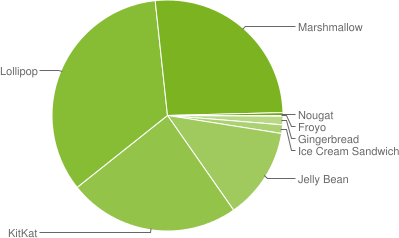
\includegraphics[width=0.9\textwidth]{androidversionchart}
 		 \captionof{figure}{Android OS fragmentation chart}
 		\label{2.2:Android fragmentation chart}
 		
 	\end{minipage}
 ~\hfill~
 \begin{minipage}{0.5 \textwidth}
 	\centering
 	\begin{tabular}{lll}
 		%
 		\toprule
 		%
 		\textbf{Version}  & \textbf{API Level} & \textbf{Distribution}\\
 		%
 		\midrule
 		%
 		2.2 & 8 & 0.1\% \\
 		2.3.3 - 2.3.7 & 10 & 1.2\% \\
 		4.0.3 - 4.0.4 & 15 & 1.2\% \\
 		4.1.x & 16 & 4.5\% \\
 		4.2.x & 17 & 6.4\% \\
 		4.3 & 18 & 1.9\% \\
 		4.4 & 19 & 24.0\% \\
 		5.0 & 21 & 10.8\% \\
 		5.1 & 22 & 23.2\% \\
 		6.0 & 23 & 26.3\% \\
 		7.0 & 24 & 0.4\% \\
 		%
 		\bottomrule
 		%
 	\end{tabular}
\end{minipage}
 	%
 \end{table}
Data in \tablename~\ref{tab:chart} were collected during a 7-day period ending on December 5, 2016, by Google. Any versions with less than 0.1\% distribution are not shown \cite{devandroiddash}.
\subsection{Structure}
\par
Android is an operating system based on the Linux kernel. The project responsible for developing the Android system is called the \textit{Android Open Source Project (AOSP)} and it lead by Google.
\begin{figure}[h]
	\centering
	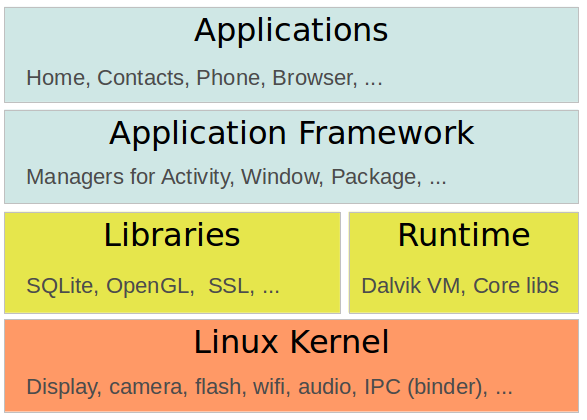
\includegraphics[width=0.8\textwidth]{oslevels}
	\caption{Android OS 4 layers}
	\label{fig:2.3}
\end{figure}

The OS can be divided into the four layers as depicted the \figurename~\ref{fig:2.3}. An Android application developer typically works with the two layers on top to create new Android applications \cite{vogel2016android}.

\paragraph{Linux Kernel} is the most flexible operating system that has ever been created. It can be tuned for a wide range of different systems, running on everything from a radio-controlled model helicopter, to a cell phone, to the majority of the largest supercomputers in the world \cite{hartman2006linux}. This is in practice the communication layer for the underlying hardware.
\paragraph{Runtime}  is the term used in computer science to designate the software that provides the services necessary for the execution of a program.There are two different \textit{"runtime systems"} which can work with the Android OS:
\begin{itemize}
	\item \textit{Dalvik VM} is an optimized version for low memory devices of the \textit{Java Virtual Machine (JVM)} used Android 4.4 and earlier version. It is stack based and it works by converting, each time an application it is executed, Android's \textit{bytecode} in machine code.
	\item \textit{ART (Android Runtime)} introduced with Android 4.4 KitKat. This runtime uses an \textit{AOT (Ahead-of-Time)} approach, with which code is compiled during the installation of an application an then is ready to be executed.
\end{itemize}
\paragraph{Application Framework}
\paragraph{Applications}


 
\section{Distributed System} \label{distsys}
\subsection{Definition}

\subsection{Examples} \label{distex}


\section{Liquid Computation}
\subsection{Definition}
\par 




I have only quickly listed some features and possible issues of my source, to have a complete idea it is possible to read all the proposed solutions and ideas in \cite{guinard2011web}.
%
% ------------------------------------------------------------------------ %6